\section{Моделирование робота}
\subsection{ZenCad}
В качестве CAD программы для моделирования деталей робота и создания цифрового двойника была выбрана библиотека параметрического 3d моделирования ZenCad. Автор библиотеки вдохновлен программой OpenScad, проектирование в котором заключалось в написании скрипта, являющегося инструкцией для графического ядра, строящего модель. Без интерактивных инструментов изменения объектов. В ZenCad используется ядро граничного представления OpenCascade, что является преимуществом по сравнению с OpenScad, использующим математику полигональных сеток. Необходимость представлять каждую модель, как массив полигонов приводит к комбинаторному взрыву, при усложнении сцены, что в свою очередь заставляет разрабатывать модели с меньшим разрешением, чем их финальный вид, ради экономии вычислительных ресурсов. Особенностью граничного представления твёрдого тела заключается в описании модели, как набора поверхностей, с заданной точностью соединенных по границам и образующих замкнутый объем. То-есть окружность задается не как многоугольник с заданным количеством вершин, а именно как функция окружности, задаваемая двумя точками: центром и точкой на окружности, соответствующей 0 радиан. Подобное представление позволяет определять объем тела и его массово-инерционные характеристики, а также упрощает его разбиение на конечные элементы для инженерного анализа (так как можно легко определить, лежит ли точка внутри тела или за его пределами). Для удобства работы параметрические модели представляются в виде логического дерева построения. Фактически, каждая геометрическая операция (вытянуть, построить по сечениям и др.) – это набор алгоритмов, создающих набор корректно связанных поверхностей. При изменении компонента дерева построения все последующие элементы будут перестроены. Если при этом исчезнут элементы, к которым были привязаны последующие построения, то модель окажется некорректной. Поэтому, проектируя изделие, необходимо четко представлять иерархию дерева и возможные способы последующего изменения геометрии.

Для ускорения расчетов сцены используется библиотека ленивых вычислений evalcache для агрессивного кэширования вычислений. Объекты, параметры которых не были изменены будут исключены из расчетов и загружены из кэша. В том числе и одинаковые объекты сцены не будут обсчитываться несколько раз. Ради демонстрации моделей с разными значениями параметров, можно заранее их обсчитать и соответственно разные версии модели будут храниться в кэше. В теории возможно переносить папку кэша с одного компьютера на другой, если это целесообразно (очень сложный проект и маломощный компьютер). С другой стороны, моделирование в ZenCad представляет собой программирование, то-есть изменение текстового документа, для чего возможно использовать любой компьютер и текстовый редактор.

Созданный мной цифровой двойник представляет собой программу на языке <<Python>>, текст которой разделён на три логических секций:

\paragraph{Константы} здесь размещены все константы, используемые в скрипте и их часто используемые отношения, для облегчения расчетов и экономии места.
\paragraph{Функции} для удобства работы с деталями робота, все они создаются в виде функций, к которым происходит обращение в нужный момент. К некоторым функциям, бывают обращения внутри других функций, например, для выреза под гайку, которая используется в нескольких деталях.  
\paragraph{Интерактивные объекты и анимация} особенностью ZenCad является то, что сами по себе модели не будут присутствовать в сцене до тех пор, пока не будут превращены в интерактивные объекты. Есть несколько способов создания интерактивных объектов, я использую функцию n = disp(m), которая из объекта, хранящейся в переменной m, создает интерактивный объект n. В случае с анимацией, если координату куба представить в виде массива из 10 значений, то в сцене будет генерироваться 10 кубов. Для создания анимации, необходимо менять координату именно интерактивного тела, что делается с помощью специальных функций. 


\subsection{База}

База представляет собой основную конструкционную часть робота, задающей конструкционную жесткость для всех остальных элементов конструкции. Основной сложностью для  создания дельта робота, заключается в необходимости с большой точностью располагать рычаги под углом в $120^{\circ}$ друг к другу. От точности углов, чрезвычайно сильно зависит возможность управления роботом в дальнейшем. К счастью, 3д печать, как и ЧПУ фрезеровка, позволяет обойти эту сложность, убирая человеческий фактор, так как расположение всех креплений и отверстий задается станком с высокой точностью. В следствие моего решения печатать все детали робота на 3д принтере, я обязан уместить их в рамках печатной поверхности своего принтера, а именно в квадрат 20х20 сантиметров. Так как база не умещается в данные габариты, мне пришлось сделать ее разборной. Центральная цилиндрическая часть имеет 3 паза под ласточкин хвост, в которые встают "лепестки" с креплением для двигателей, червячного редуктора, концевиков и оси рычага.

\paragraph{Ласточкин хвост} для создания которого используется возможность построения многоугольника polygon по массиву pnts, состоящего из координат точек. Первым делом происходит проверка флага f на True/False, что символизирует будет ли данных объект непосредственно ласточкиным хвостом или пазом под него. Это важно, так как паз должен иметь зазор, определяемый переменной dh. Зазор подобран экспериментально, напечатанные детали имеют достаточно шершавые поверхности, в следствие послойного наплавления. При данном зазоре одна деталь с трудом стыкуется с другой и держится силой трения. При объявлении двумерного массива pnts, я вносил координаты в формате [[1,2],[3,4]] которые автоматически воспринимаются как 2 координаты Х и У, фигура соответственно получается плоской и в плоскости ХУ. Если бы стояла задача использовать все три координаты их можно было записывать как [[1,2,3],[4,5,6]]. После получения плоской фигуры (трапеции), происходит ее экструдирование с помощью функции linear\_extrude() на вектор vec=(0,0,20).         

\begin{verbatim}
    def hvost(f): # Ласточкин хвост
        if f == 1 :
            dh = 0.3
        else:
            dh = 0
        pnts=      [[ 20 + dh , 10  + dh],
                    [ 10 + dh , -10 - dh],
                    [-10 - dh , -10 - dh],
                    [-20 - dh , 10  + dh]]
        o=polygon(pnts=pnts,wire=False)
        m=linear_extrude(proto=o,vec=(0,0,20),center=True)
    return m
\end{verbatim}

\paragraph{Вырез под гайку} позволяет упростить процесс сборки и симпатично спрятать гайки внутри конструкции. Сам по себе, он имеет форму шестигранного цилиндра. Для создания шестигранника используется специальная функция ngon() с параметром n (количество граней) равным шести. Параметр wire отвечает за то, является ли двумерный объект полноценным, заполненным полигоном или только контуром. Основная сложность остается в определении радиуса. В данном случае подразумевается радиус описанной окружности многоугольника. Если измерить гайку штангель-циркулем, то получится диаметр вписанной окружности шестиугольника. Так как в шестиугольнике радус описанной окружности относится к радиусу вписанной как $sin(60^{\circ})$, получаем соотношение:

\begin{center}
    $r_{ngon} = \frac{0.5*2}{\sqrt{3}}*d_{gaika} + dh_{zazor}$
\end{center}

Итоговая величина зазора подбиралась экспериментально, чтобы гайка входила в гнездо плавно и не выпадала под собственным весом. Конкретно $dh=0.225$

\begin{verbatim}
    def pos_gaiki(): # функция выреза под гайку
        m = ngon(r=4.15,n=6,wire=False)
        n = linear_extrude(proto=m, vec=(0,0,5), center=True)
    return n
\end{verbatim}

\paragraph{Центральная часть робота} помимо скрепления "лепестков" также имеет важную функцию крепления дельта-робота к его рабочему месту. В данном случае, так как стояла задача создания макета робота, была создана легкая рама из алюминиевого квадратного профиля, непосредственно стыкуемого с центральным элементом робота. В его рабочей версии, крепление придется значительно переработать.
Для нейро-сетевого процесса управлением роботом, в базе предусмотрено посадочное место для расположения камеры точно по центру.  
 
\begin{figure}[h!]
	\centering
	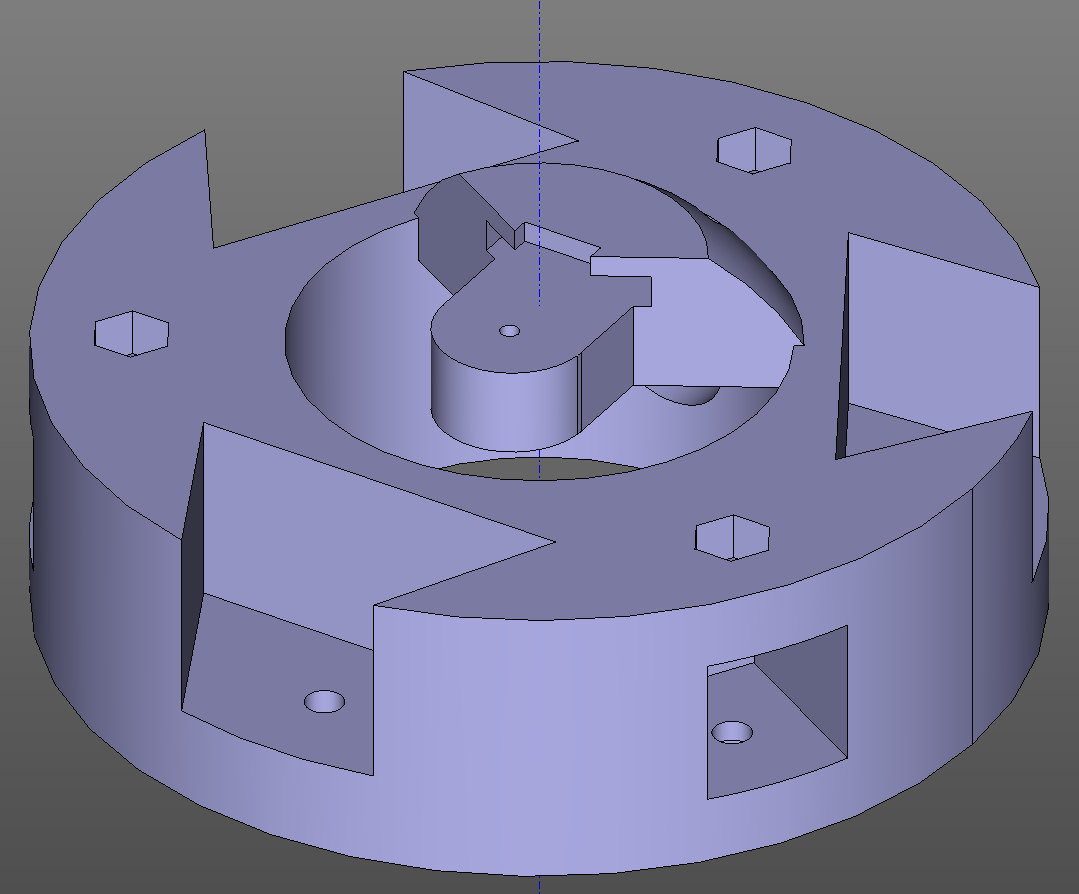
\includegraphics[width=0.8\linewidth]{./image/baza}
	\caption{Центральная деталь дельта-робота}
\end{figure} 

Все крепления осуществляются винтами М4 с шляпками под внутренний шестигранник и самоконтрящимися гайками.

\paragraph{Лепесток} отвечает за один из важнейших параметров дельта-робота, а именно за радиус базы, переменную rad. Изменение радиуса базы (расстояние от центра робота, до одной из осей вращения рычагов) меняется за счет изменения длинны данной детали. В данном случае, предоставлено значение rad = 150 милиметров, которое можно считать предельным значением. Минимальным значением можно считать 90 миллиметров, если не менять конфигурацию центральной части. При значениях меньше 90 мм., целесообразно печатать базу единой деталью.   

\begin{figure}[h!]
	\centering
	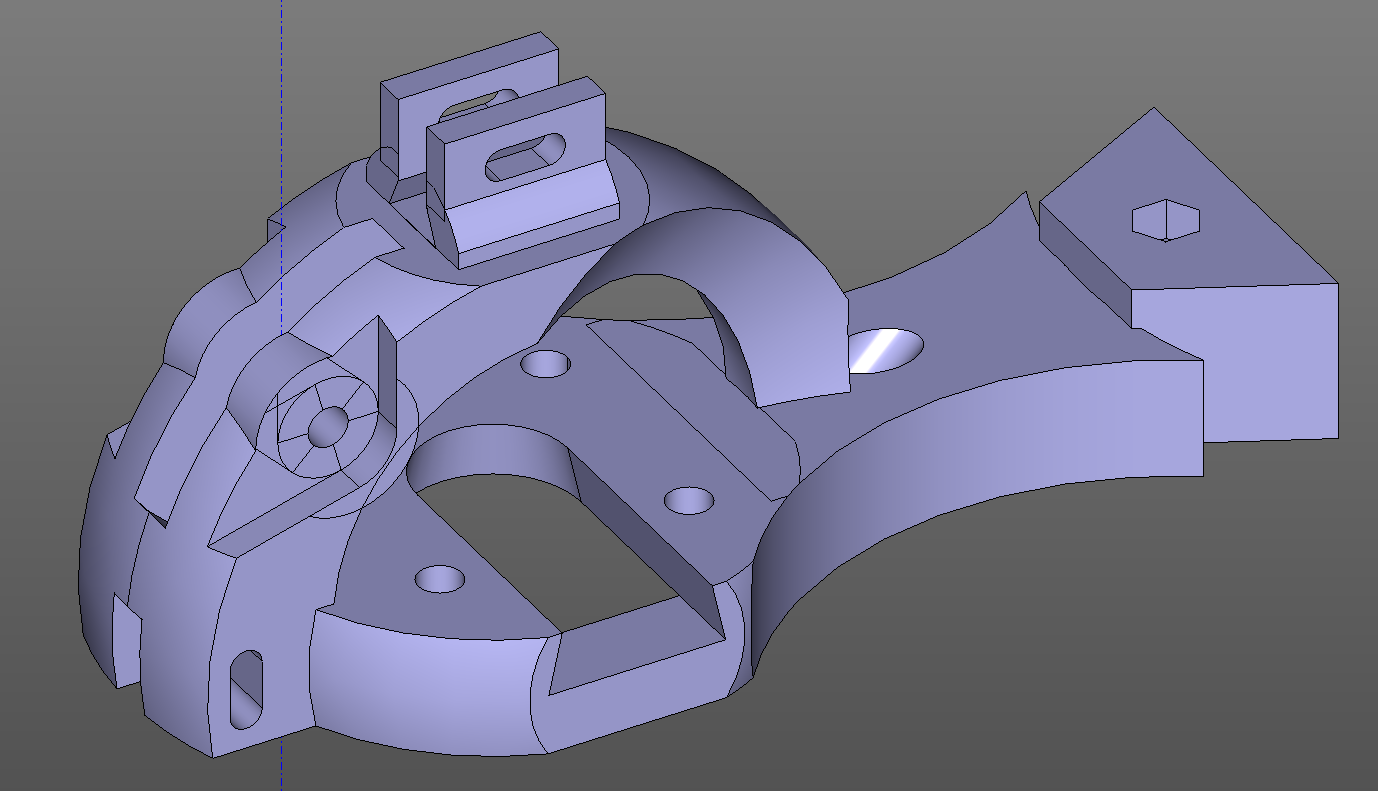
\includegraphics[width=0.8\linewidth]{./image/lepestok}
	\caption{Вторая деталь базы дельта-робота}
\end{figure} 

Для увеличения жесткости напечатанной детали, желательно придавать ей как можно больше сложных криволинейных поверхностей. В данном случае использовано максимальное количество сферических поверхностей. Все прямоугольные поверхности проектировались по принципу пересечения сферы с кубом, или вычитания сфер из формы. 

\begin{verbatim}
     krep = box((xz_dvig+20,xz_dvig+20,15),center=True)\
            ^ sphere(r=0.8*xz_dvig)
\end{verbatim}

В частности главная центральная часть данной детали (крепеж шагового двигателя), это прямоугольный параллелепипед со сторонами Х и У на 20 миллиметров больше, чем габариты двигателя, и  Z стороной равной 15 мм. С помощью оператора $\wedge$ находится пересечение со сферой радиусом 80 $\%$ от величины габаритов двигателя. Таким образом вместо прямоугольных форм получаются округлые,  способные противостоять большим скручивающим нагрузкам. Расположенная перпендикулярно арка также представляет собой полусферу, пересеченную с кубоидом. Пространство под аркой представляет собой вычтенную сферу, так как располагающийся там глобоидный червь тоже имеет габариты сферы. В следствие этого, края арки находятся немного ниже высоты червя, и тот на свое место встает с щелчком, за счет упругости пластика. Это один из способов удержания червя, использованный тут.
У каждого лепестка есть два настраиваемых крепления для концевиков, позволяющие немного регулировать крайние положения рычага. При настройке робота крайне важно выставить рычаги в начальные позиции (в моем случае это $-15^{\circ}$) и для облегчения настройки, есть физическое ограничение для поворота рычага соответствующие положениям $-15^{\circ}$ и $90^{\circ}$. Таким образом, выставив рычаг в одно из крайних положений, есть возможность отрегулировать позицию концевика на срабатывание в нужный момент. 

\subsection{Глобоидная червячная передача}

Глобоидная червячная передача является разновидностью червячных передач, когда зона механического соприкосновения червя и колеса изогнута по вогнутой (глобоидной) траектории. Это обеспечивает большое сцепление по количеству зубьев, в сравнении с обычной передачей в несколько раз в зависимости от конфигурации количества зубьев и диаметра колеса. В промышленных механизмах данная передача используется редко из-за некоторых минусов связанных со сложностью изготовления и настройки глобоидной передачи. Также её характерной особенностью является повышенное тепловыделение, а следовательно повышенный износ и сниженный КПД, в сравнении с цилиндрическим червём. Тем не менее, в данной конструкции глобоидная передача позволит сильно сэкономить пространство и расходуемый пластик.

\paragraph{Двумерное шестеренчатое колесо} является необходимым элементом, для выбранного мной способа моделирования червя. Идея построения заключается в том, чтобы взять некую форму заготовки (цилиндр или в моем случае полусферу) и, поворачивая ее вокруг своей оси, вычесть из нее форму шестеренчатого колеса, которая при этом сама поворачивается вокруг собственной оси. Таким образом, можно быть точно уверенным, что моделируемый червь и колесо идеально подходят друг к другу.

Поэтому, в первую очередь, предстояло выбрать форму шестеренчатого колеса. Самая простая форма для зубьев (если не рассматривать процесс изготовления, а с точки зрения воображения) это зубья сферической формы. Рассмотрим функцию построения двумерной шестерни из окружностей. Так как необходимые значения шага резьбы и количества зубьев изначально не определены, функция должна генерировать шестерню с произвольными значениями этих переменных. Данные две переменные являются одними из основных и вынесены в первый блок проекта. Называются teeth (количество зубов зубчатого колеса) и step (шаг резьбы червячной передачи). 

\begin{figure}[h]
	\centering
	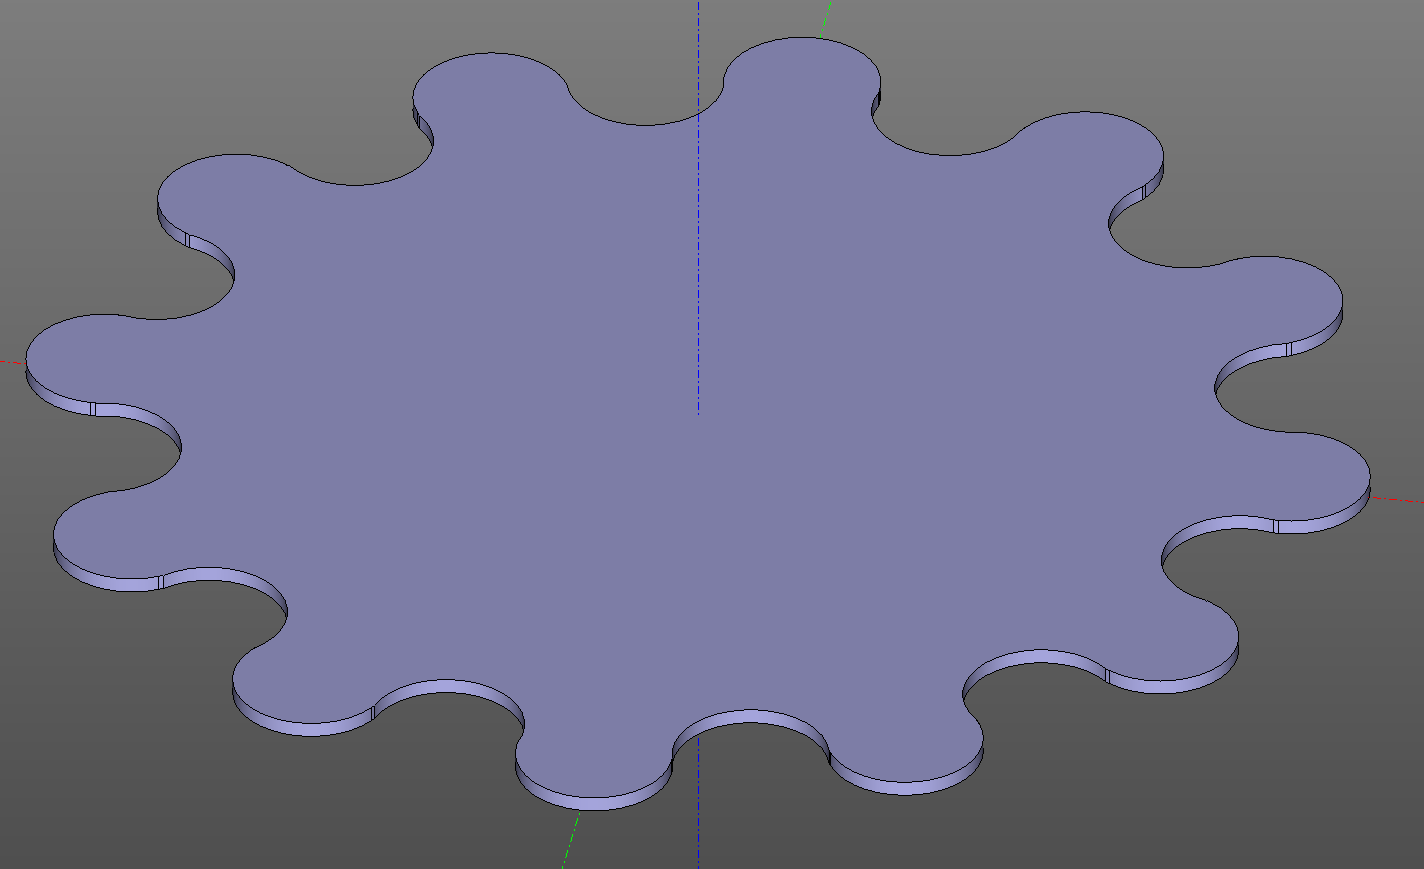
\includegraphics[width=0.8\linewidth]{./image/gear}
	\caption{Пример работы функции (добавлен объем)}
\end{figure} 

\begin{verbatim}
def gear(teeth,step): # Функция шестерни
    angle = pi/teeth
    rad_opis = (step/2) / math.sin(angle/2)
    rad_vpis = (step/2) / math.tan(angle/2)
    c=[]
    def c1(i): # Функция зуба колеса
        a  = i*2*angle
        c1 = circle(step/2,angle=(1.5*pi,0.5*pi), wire=True)\
            .moveX(rad_opis).rotateZ(a)
        return c1
    def c2(i): # Функция впадины колеса
        a  = i*2*angle
        c2 = circle(step/2,angle=(0.5*pi,1.5*pi), wire=True)\
             .moveX(rad_vpis).rotateZ(a+angle)
        return c2
    for i in range(teeth):
        o = sew([c1(i),\
                segment(c1(i).endpoints()[-1],c2(i).endpoints()[-1]),\
                c2(i)  ])
        p = segment(c2(i).endpoints()[0], c1(i+1).endpoints()[0])
        c.append(o)
        c.append(p)
    return sew(c)
\end{verbatim}

Основная задача данной функции заключается в том, чтобы расставить половинки окружностей определенным образом в пространстве. Для формирования формы шестеренчатого колеса, можно представить многоугольник в вершинах которого расположены центры окружностей зубьев, а серединах сторон - центры окружностей, вырезающие впадины. Количество вершин многоугольника будет соответствовать количеству зубьев колеса (teeth), а сторона - шагу резьбы (step). 

Внутри функции объявлены две отдельные функции c1(i) и c2(i) для построения i-той половинки окружности зуба и впадины соответственно. А внутри них располагается функция circle(), которая имеет 3 параметра: радиус окружности, угол (angle), с помощью которого создается не окружность целиком, а дуга, ограниченная начальным и конечным углом, и wire - является объект контуром или сегментом. Радиус окружностей равен половине шага резьбы. Чтобы поместить цент окружности во все вершины многоугольника, нужно один раз сместить его на радиус описанной окружности и teeth раз повернуть на удвоенный угол angle. Таким образом используется удобство полярных координат. Для впадин аналогично, но переместить нужно на радиус вписанной окружности. Оба радиуса и угол находятся с помощью тригонометрии в самом начале.

Самое сложное в данной функции - это получение из разрозненных кусочков, единый двумерный объект. Для соединения нескольких линий в одну, существует функция sew([line1,line2]), которая обрабатывает массивы, состоящие из линий. Соответственно, необходимо объявить массив c=[] и циклично добавлять в него полуокружности, чтобы потом объединить их в единое целое. К сожалению, в месте, где должны соединяться полуокружности рядом находится большое количество точек, и алгоритм функции sew() не способен самостоятельно решить, какие точки необходимо скреплять, поэтому ему необходимо помочь. Необходимо воспользоваться функцией segment(point1, point2), которая создает отрезок, соединяющий точки point1 и point2. В качестве точек нужно взять граничные точки линий, для чего существует преобразование line.endpoints()[0], где 0 - это номер точки объекта line. Конечно, таким образом можно обратиться к любой точке, из которой состоит линия, но как обратиться к последней точке? Так как линия является массивом из точек, то задача состоит в обращении к последнему элементу массива, номера которого мы не знаем. В python мы можем это сделать, вызвав переполнение, то-есть обратившись к -1 элементу массива.

В контексте данной задачи, линия O представляет собой сумму зуба, впадины и отрезка, соединяющих их последние точки. Линия P представляет собой отрезок, соединяющий первую точку впадины с первой точкой следующего зуба. Когда цикл teeth раз добавит эти линии к массиву с, будет возможно полностью объединить массив в одну линию и вернуть её, как результат работы функции - return sew(c). Обращаю внимание, что алгоритм делает все операции за один цикл 

В данном случае явно продемонстрированы сложности, связанные с тем, что ZenCad использует ядро граничного представления. В случае с OpenScad мелкие погрешности несовпадения точек в пространстве, были бы нивелированы, представлением окружностей, как многогранников с четко определенными величинами минимальных деталей. В ZenCad даже ничтожный разрыв линии превратит замкнутую фигуру в незамкнутую, за чем необходимо очень пристально следить. Так как к незамкнутым фигурам нельзя применить те операции, которые необходимо сделать в дальнейшем.

\paragraph{Создание тора из вращающейся шестерни} Если взять полученную выше шестерню и замкнуть её в трёхмерный тор, параллельно поворачивая её вокруг своей оси, то можно получить форму, обратную форме червя. Достаточно будет вычесть этот тор из сферы или цилиндра, чтобы получить конечную форму глобоидного червя. Задача состоит в том, чтобы разработать алгоритм построения данной фигуры и, так как её расчёт будет достаточно затратным для вычислительных мощностей, распараллелить вычисления, благо python предлагает инструменты для этого. 

Для распаралелливания вычислений используется модуль futures. Идея заключается в том, чтобы фигуру, похожую на тор, разделить на 4 равные части и рассчитывать эти части параллельно в 4 потока. 
\begin{figure}[h]
	\centering
	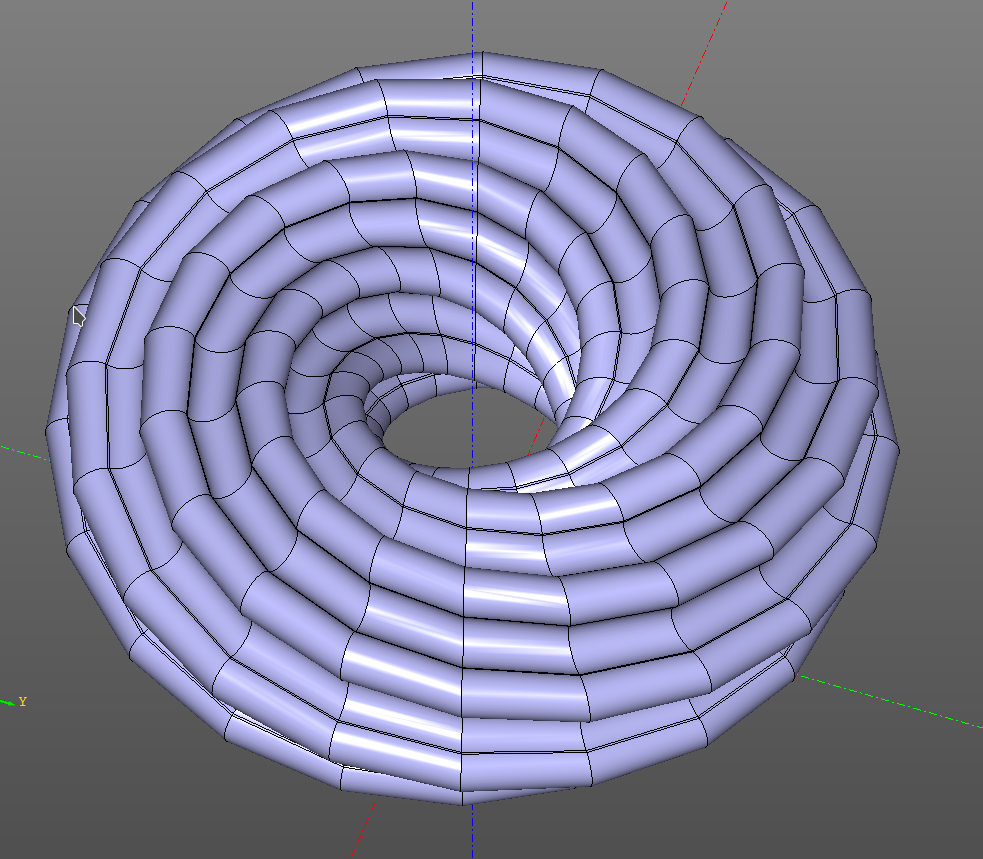
\includegraphics[width=0.8\linewidth]{./image/worm_tor}
	\caption{Обратная форма глобоидного червя}
\end{figure} 

\begin{verbatim}
from concurrent import futures
def worm (): # Червь
    angle = pi/teeth
    rad_opis =(step/2) / math.tan(angle/2)
    a = (n_s*angle*0.5)/n
    b = 0.5*pi/n
    def chast(x):
        if x==
                da = 0
                db = 0
        if x==1:
                da = a*n
                db = pi/2
        if x==2:
                da = 2*a*n
                db = pi
        if x==3:
                da = 3*a*n
                db = 1.5*pi
        g=[]
        r=0.5*(xz_dvig+10)
        for i in range(n+1):
                g.append(gear(teeth,step).rotateY(i*a + da)\
                            .translate(r,0,20).rotateZ(i*b + db))
        w = loft(g)
        return w
    x = [i for i in range(0,4,1)]
    with futures.ThreadPoolExecutor() as executor:
        worm = executor.map(chast, x)
 \end{verbatim}



